%=============================================================================
%  CHAPTER 4 — RELEASE 1: SPRINT 1 (FOUNDATIONS) AND SPRINT 2 (RIDES & BOOKINGS)
%=============================================================================
\chapter{Release 1: Foundations and Core Booking Workflow}

\clearpage
\section*{Introduction}

The first release of ForsaDrive groups the work carried out during Sprint~1 and Sprint~2. The objective of this release was to deliver a usable product as soon as possible, even at the cost of leaving some advanced features for the next release. Sprint~1 focused on the \textit{Foundations}: account creation, authentication, profile management, student verification, the driver application flow, and the administrative validation that controls access to the driver role. Sprint~2 then built the \textit{Rides and Bookings} workflow on top of these foundations: ride publishing, search and filtering, single and group booking, and the management of booking requests by drivers. By the end of the release, a passenger could register, become a verified student, search for a ride, and book a seat with a fifty-percent prepayment, while a driver could publish trips and review the bookings he had received.

This chapter follows the same structure for each sprint: a short presentation of the sprint backlog with the user stories that were planned, a description of the conception artifacts that were produced (sequence and activity diagrams when relevant), the realization of the corresponding screens on the web and on the mobile, and a brief sprint review. Before entering the sprints themselves, the chapter opens with the development environment and the technological choices that were retained for the entire project, since these decisions affect every later sprint and would clutter the discussion if repeated each time.

\section{Development Environment}

\subsection{Hardware Environment}

The platform was developed on two personal workstations used in parallel by the team. Each machine had enough resources to run the development server, the database engine, and the emulators needed during the implementation. The hardware configurations are summarized in Table~\ref{tab:hw_env}.

\begin{table}[H]
\centering
\caption{Hardware environment}
\label{tab:hw_env}
\begin{tabular}{|l|p{9cm}|}
\hline
\textbf{Component}     & \textbf{Configuration} \\
\hline
Processor              & Intel Core i5 / i7 (8th generation or later) \\
\hline
Memory (RAM)           & 8 GB to 16 GB \\
\hline
Storage                & SSD, 256 GB or more \\
\hline
Operating system       & Windows 10/11 and Ubuntu 22.04 \\
\hline
\end{tabular}
\end{table}

\subsection{Software Environment}

The tools used during the project were chosen for their availability, the experience already acquired by the team during the training, and their compatibility with the technological stack. Table~\ref{tab:sw_env} lists the main ones.

\begin{table}[H]
\centering
\caption{Software environment and tooling}
\label{tab:sw_env}
\begin{tabular}{|l|p{9.5cm}|}
\hline
\textbf{Tool} & \textbf{Role in the project} \\
\hline
Visual Studio Code & Main editor for backend and Flutter, with PHP and Dart extensions. \\
\hline
XAMPP / Apache & Local server stack hosting the PHP backend during development. \\
\hline
Android Studio + emulator & Compilation of the Flutter app and execution on virtual devices. \\
\hline
Git and GitHub & Version control and code sharing between the two team members. \\
\hline
Postman & Manual and collection-based testing of the REST API. \\
\hline
DB Browser for SQLite & Inspection and ad-hoc queries on the SQLite database. \\
\hline
PlantUML & Production of the UML diagrams included in the report. \\
\hline
Trello & Lightweight tracking of the sprint backlog and the daily progress. \\
\hline
\end{tabular}
\end{table}

\section{Technologies Used}

The technological choices made at the beginning of the project apply to every sprint. They were driven by three considerations: the constraints of the project, the experience already acquired during the training at the institute, and the standards adopted by the host organization.

\subsection{Frontend Technologies (Web)}

The web interface is built with PHP rendered server-side, combined with HTML5 and Bootstrap~5 for layout and styling. PHP handles routing, session management, and page rendering in a unified server-side model, which avoids the complexity of a separate frontend build step. Bootstrap was chosen for its responsive grid system and for the consistency it brings to a large set of UI components --- forms, modals, tables, navigation bars --- across the many pages of the application. Client-side interactivity is handled with plain JavaScript, without any additional framework. Dynamic behaviors such as form validation, tab switching in the administration panel, and asynchronous calls for real-time feedback are implemented in small, focused scripts.

\subsection{Backend Technologies}

The backend business logic is written in PHP and exposed as a REST API under the \texttt{/api/} route prefix. PHP was selected because the host organization already operates a PHP-based infrastructure, the language is natively supported by XAMPP without any additional runtime, and the team had prior experience with it. The API follows a front-controller pattern: a single \texttt{index.php} entry point parses the URL, dispatches the request to the appropriate handler file, and returns a JSON response. Database access is performed through PDO with parameterized queries, which protects the application against SQL injection.

Authentication relies on randomly generated bearer tokens stored in an \texttt{api\_tokens} table. After a successful login, the server creates a 32-byte hex token with a 30-day expiry and returns it to the client. Every protected endpoint validates the token from the \texttt{Authorization} header and rejects requests that carry an expired or unknown token.

\subsection{Mobile Technology --- Flutter}

Two main options were considered for the mobile application: developing natively for Android and iOS on the one hand, or using a cross-platform framework on the other. Native development would have doubled the effort without providing enough additional value for a ride-sharing use case, so a cross-platform framework was preferred. After a short evaluation against the time budget of the internship and the team's experience, \textbf{Flutter} was selected.

Flutter is an open-source UI toolkit maintained by Google that allows a single Dart codebase to compile into native applications for Android and iOS. Unlike JavaScript-based frameworks that bridge to native components at runtime, Flutter draws its own widgets using the Skia rendering engine, which gives it pixel-perfect consistency across platforms and a very smooth scrolling behavior. The hot-reload feature also significantly accelerated the iterative work during the sprints. Several supporting packages were added on top of the framework: \texttt{go\_router} for declarative navigation, \texttt{provider} for ChangeNotifier-based state management, \texttt{http} for the REST calls, \texttt{shared\_preferences} for the local persistence of the session token and the language, \texttt{flutter\_map} for the interactive map screen, \texttt{firebase\_messaging} for push notifications, and \texttt{flutter\_localizations} for the multilingual interface.

\subsection{Database --- SQLite}

SQLite was selected as the persistent store. It is a file-based, serverless relational database that requires no separate process, which makes it easy to set up, back up, and share between the web and mobile clients through the same shared file. The database runs in WAL (Write-Ahead Logging) mode to support concurrent reads from the mobile application while the web server writes. Indexes are placed on the columns most frequently used for filtering, in particular the origin, the destination, and the departure date of rides. SQLite is acknowledged as a development choice; the limitations of this option for a high-traffic production environment are discussed in the general conclusion.

\section{Sprint 1 --- Foundations}

\subsection{Sprint Goal and Backlog}

Sprint~1 was planned to last roughly three weeks. Its goal was the one most often quoted in Scrum literature: to deliver an environment in which a real user can be created and can authenticate. Without this, no further sprint can be reviewed against actual interactions. The user stories that were placed in the sprint backlog are listed in Table~\ref{tab:sprint1_backlog}. Story points are estimated according to the standard Fibonacci scale.

\begin{table}[H]
\centering
\caption{Sprint 1 backlog}
\label{tab:sprint1_backlog}
\begin{tabular}{|c|p{8.5cm}|c|}
\hline
\textbf{ID} & \textbf{User story} & \textbf{Points} \\
\hline
US1.1 & As a guest, I want to register an account so that I can access the platform. & 5 \\
\hline
US1.2 & As a registered user, I want to log in with my email and password so that I retrieve my session. & 3 \\
\hline
US1.3 & As a user, I want to view and update my profile so that my information stays accurate. & 3 \\
\hline
US1.4 & As a passenger, I want to verify my student status through a university email OTP so that I receive the student discount. & 8 \\
\hline
US1.5 & As a passenger, I want to apply to become a driver by submitting my license and vehicle so that I can publish trips. & 8 \\
\hline
US1.6 & As an admin, I want to review and approve or reject driver applications so that only verified drivers can publish rides. & 5 \\
\hline
US1.7 & As an admin, I want to manage the list of recognized university domains so that the OTP flow remains under control. & 3 \\
\hline
\end{tabular}
\end{table}

\subsection{Detailed Conception}

Two flows from this sprint are sensitive enough to deserve their own sequence diagrams: the self-service student verification, because it involves the email channel and a strict expiration policy, and the driver application with admin approval, because it changes the role of the user and creates side effects on multiple tables.

\begin{figure}[H]
    \centering
    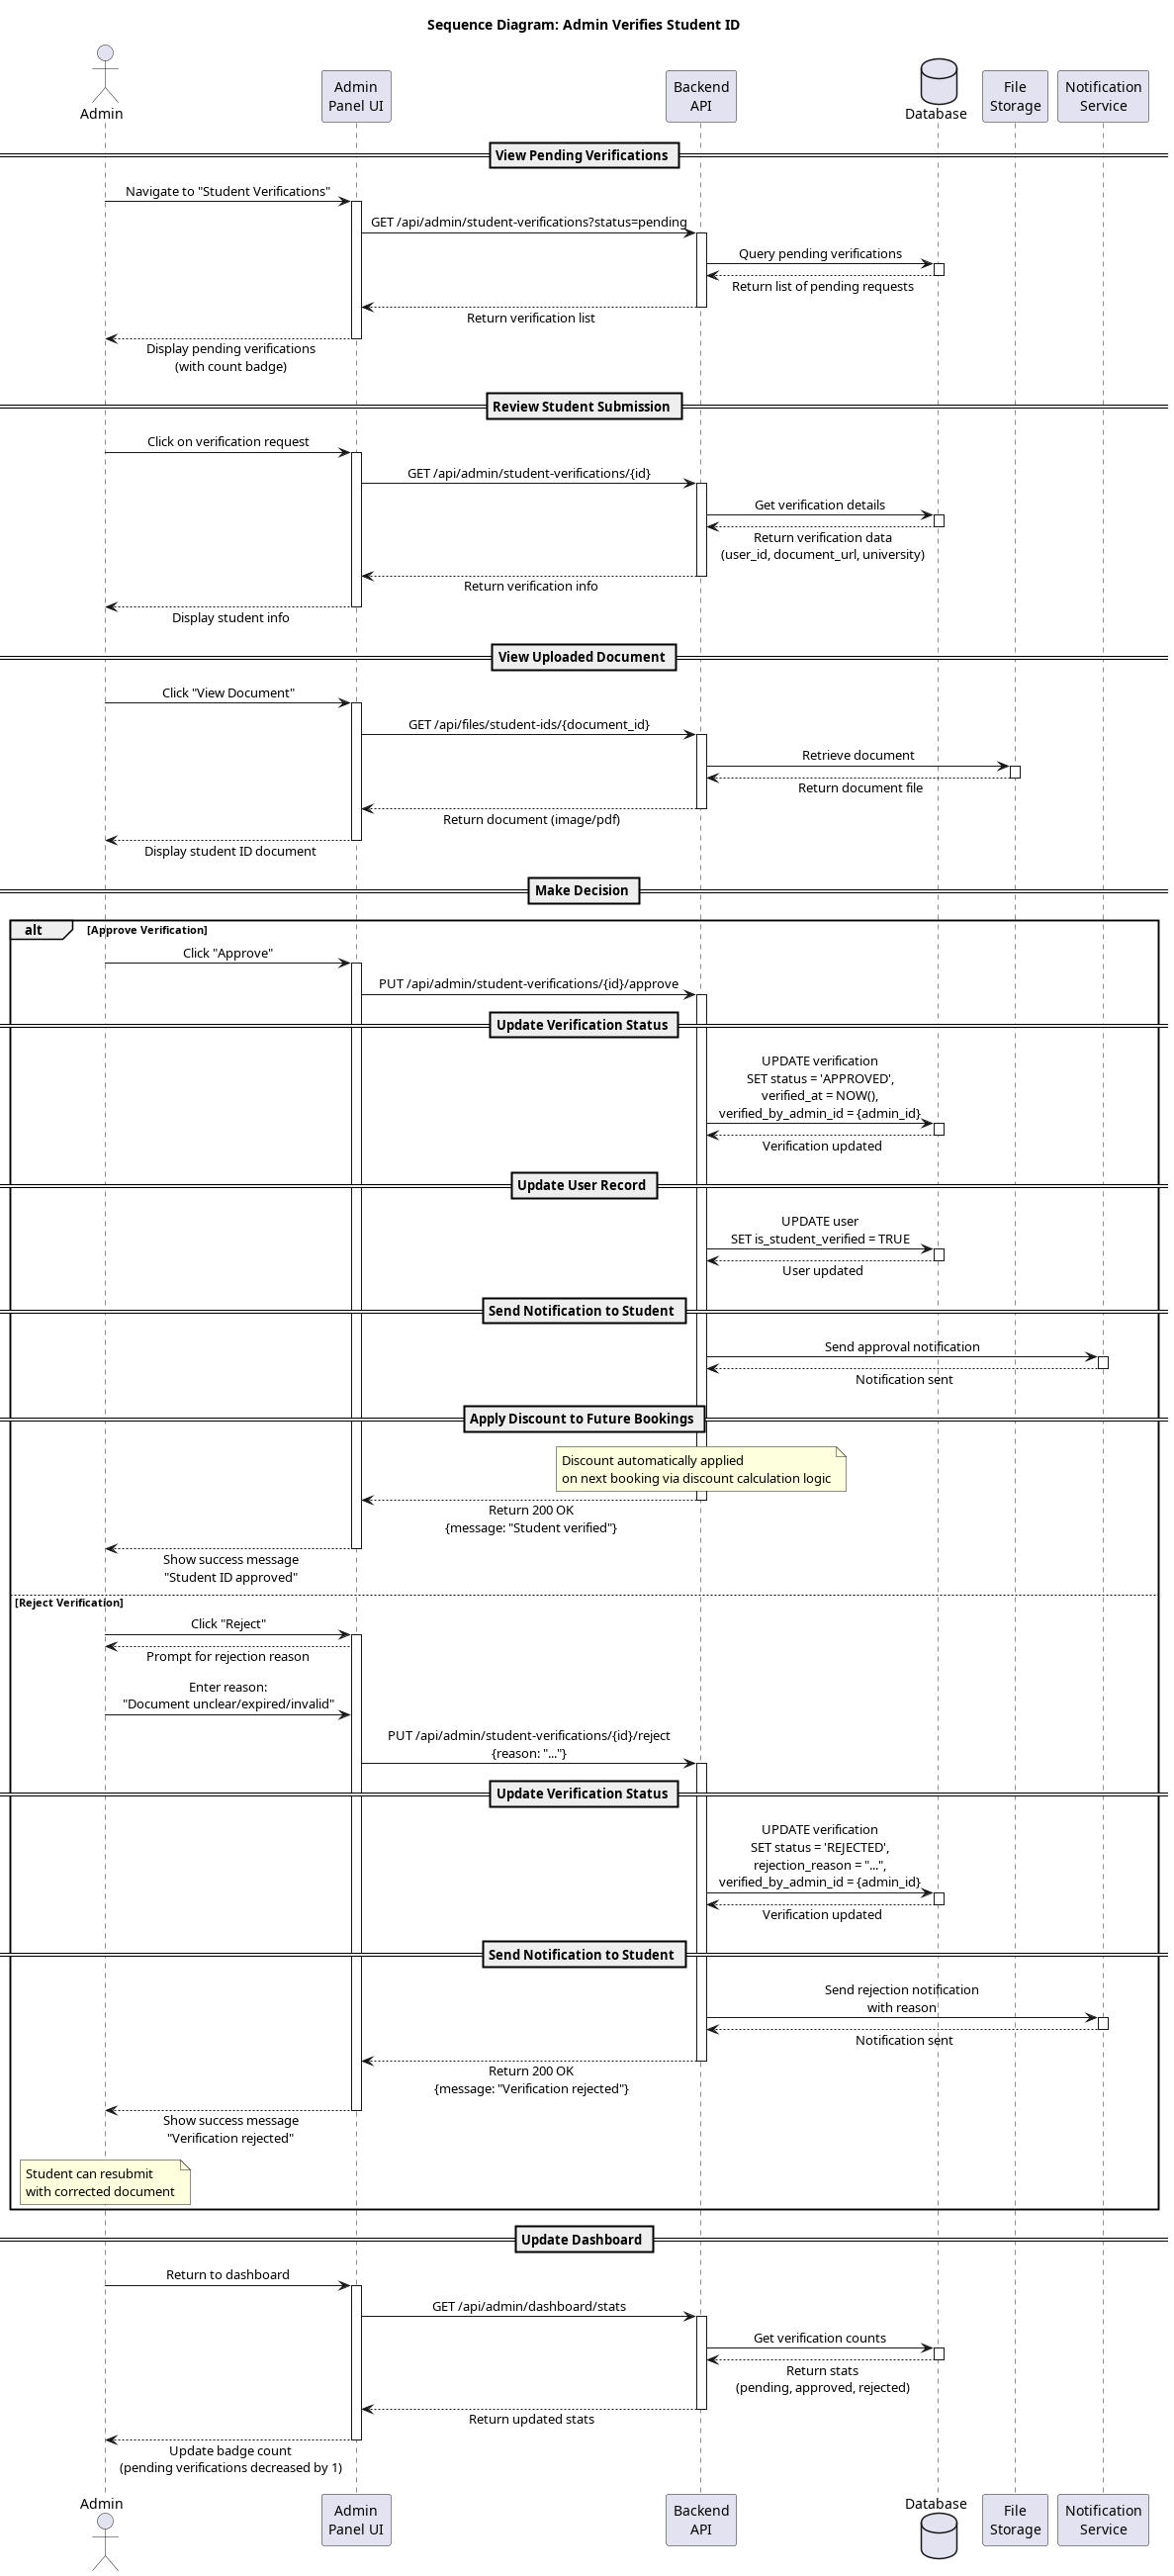
\includegraphics[width=\textwidth, height=0.85\textheight, keepaspectratio]{ForsaDrive_Sequence_VerifyStudent.png}
    \caption{Sequence diagram --- self-service student OTP verification (US1.4)}
    \label{fig:seq_otp_verify}
\end{figure}

The student verification flow opens when the passenger submits a university email address. The backend first checks that the domain is part of the active \texttt{student\_domains} table; if it is not, the user is shown the list of accepted institutions and the request stops there. If the domain is valid, a six-digit code is generated, hashed, and stored together with a ten-minute expiry. The code is then dispatched to the email address. When the user enters the received code, the backend verifies that it has not expired and that no more than five wrong attempts have been made. On success, the \texttt{is\_student\_verified} flag is set on the account and an audit row is written. The student discount is then applied automatically to any subsequent booking.

\begin{figure}[H]
    \centering
    \includegraphics[width=\textwidth, height=0.85\textheight, keepaspectratio]{ForsaDrive_Sequence_DriverApplication.png}
    \caption{Sequence diagram --- driver application and admin approval (US1.5, US1.6)}
    \label{fig:seq_driver_app}
\end{figure}

The driver application flow stores the submitted form with the status \textit{PENDING} and triggers a notification to the administrator. The admin reviews the application in the dedicated tab of the panel. On approval, the backend creates the driver profile, registers the vehicle, switches the role of the user from \textit{PASSENGER} to \textit{DRIVER}, and sends a notification back to the applicant. On rejection, the rejection reason is stored on the application row and the user remains a passenger.

\subsection{Realization}

The screens delivered at the end of Sprint~1 cover the foundations on both clients. The web application opens on a public landing page that introduces the concept and the student discount, with quick access to registration and login (Figure~\ref{fig:web_landing}). The login and registration forms perform validation on the client side for immediate feedback and confirm the inputs on the server (Figure~\ref{fig:web_auth}). The mobile application provides equivalent screens with a real-time student domain detector that highlights the email field in green when the entered address belongs to a recognized university (Figure~\ref{fig:mobile_auth}). The profile screen, common to both clients, gathers the personal information, the verification status with the student badge, and a card showing the status of any pending driver application (Figure~\ref{fig:mobile_profile}).

\begin{figure}[H]
    \centering
    \includegraphics[width=\textwidth]{web_landing.png}
    \caption{Web landing page}
    \label{fig:web_landing}
\end{figure}

\begin{figure}[H]
    \centering
    \includegraphics[width=0.85\textwidth]{web_auth.png}
    \caption{Web authentication interface}
    \label{fig:web_auth}
\end{figure}

\begin{figure}[H]
    \centering
    \includegraphics[width=0.55\textwidth]{mobile_auth.png}
    \caption{Mobile authentication --- login and registration}
    \label{fig:mobile_auth}
\end{figure}

\begin{figure}[H]
    \centering
    \includegraphics[width=0.55\textwidth]{mobile_profile.png}
    \caption{Mobile profile and student badge}
    \label{fig:mobile_profile}
\end{figure}

\subsection{Sprint Review}

The review with the supervising engineer at the end of Sprint~1 confirmed that all user stories of the sprint backlog had been completed. One remark was raised: the very first iteration of the OTP flow allowed a new code to be requested without any cooldown, which would have made the verification endpoint vulnerable to abuse. A thirty-second cooldown between two consecutive requests was added the following day, before opening Sprint~2. The retrospective also highlighted a positive practice that was kept for the rest of the project: writing the form validation rules on the backend first and then mirroring them on the client, rather than the opposite, which avoided the divergence between the two layers that had been observed on a previous course assignment.

\section{Sprint 2 --- Rides and Bookings}

\subsection{Sprint Goal and Backlog}

The goal of Sprint~2 was to deliver the central interaction loop of the platform: a driver publishes a ride, a passenger searches and books it, and the booking is confirmed by a fifty-percent prepayment. The backlog of the sprint is given in Table~\ref{tab:sprint2_backlog}.

\begin{table}[H]
\centering
\caption{Sprint 2 backlog}
\label{tab:sprint2_backlog}
\begin{tabular}{|c|p{8.5cm}|c|}
\hline
\textbf{ID} & \textbf{User story} & \textbf{Points} \\
\hline
US2.1 & As a driver, I want to publish a ride by entering its origin, destination, date, price and seats so that passengers can find it. & 5 \\
\hline
US2.2 & As a driver, I want to modify or cancel a ride that I have published so that I can adjust to last-minute changes. & 3 \\
\hline
US2.3 & As a passenger, I want to search rides by origin, destination and date so that I find the matching offers. & 5 \\
\hline
US2.4 & As a passenger, I want to filter the search results by price, departure time and driver rating so that I narrow down the offers. & 5 \\
\hline
US2.5 & As a passenger, I want to view the full details of a ride and the profile of the driver before booking. & 3 \\
\hline
US2.6 & As a passenger, I want to book one or several seats on a ride with a fifty-percent prepayment so that I confirm the booking. & 8 \\
\hline
US2.7 & As a passenger, I want to book a group seat for friends so that we travel together. & 5 \\
\hline
US2.8 & As a driver, I want to view, accept or reject the incoming booking requests for my rides. & 5 \\
\hline
US2.9 & As a passenger, I want to cancel my booking under the cancellation rules so that I am not stuck with a trip I cannot take. & 3 \\
\hline
\end{tabular}
\end{table}

\subsection{Detailed Conception}

Three diagrams are needed to describe the sprint with sufficient precision: a sequence diagram for the publication of a ride by a driver, a sequence diagram for the booking of a ride by a passenger, and an activity diagram that gives a global view of the booking journey.

\begin{figure}[H]
    \centering
    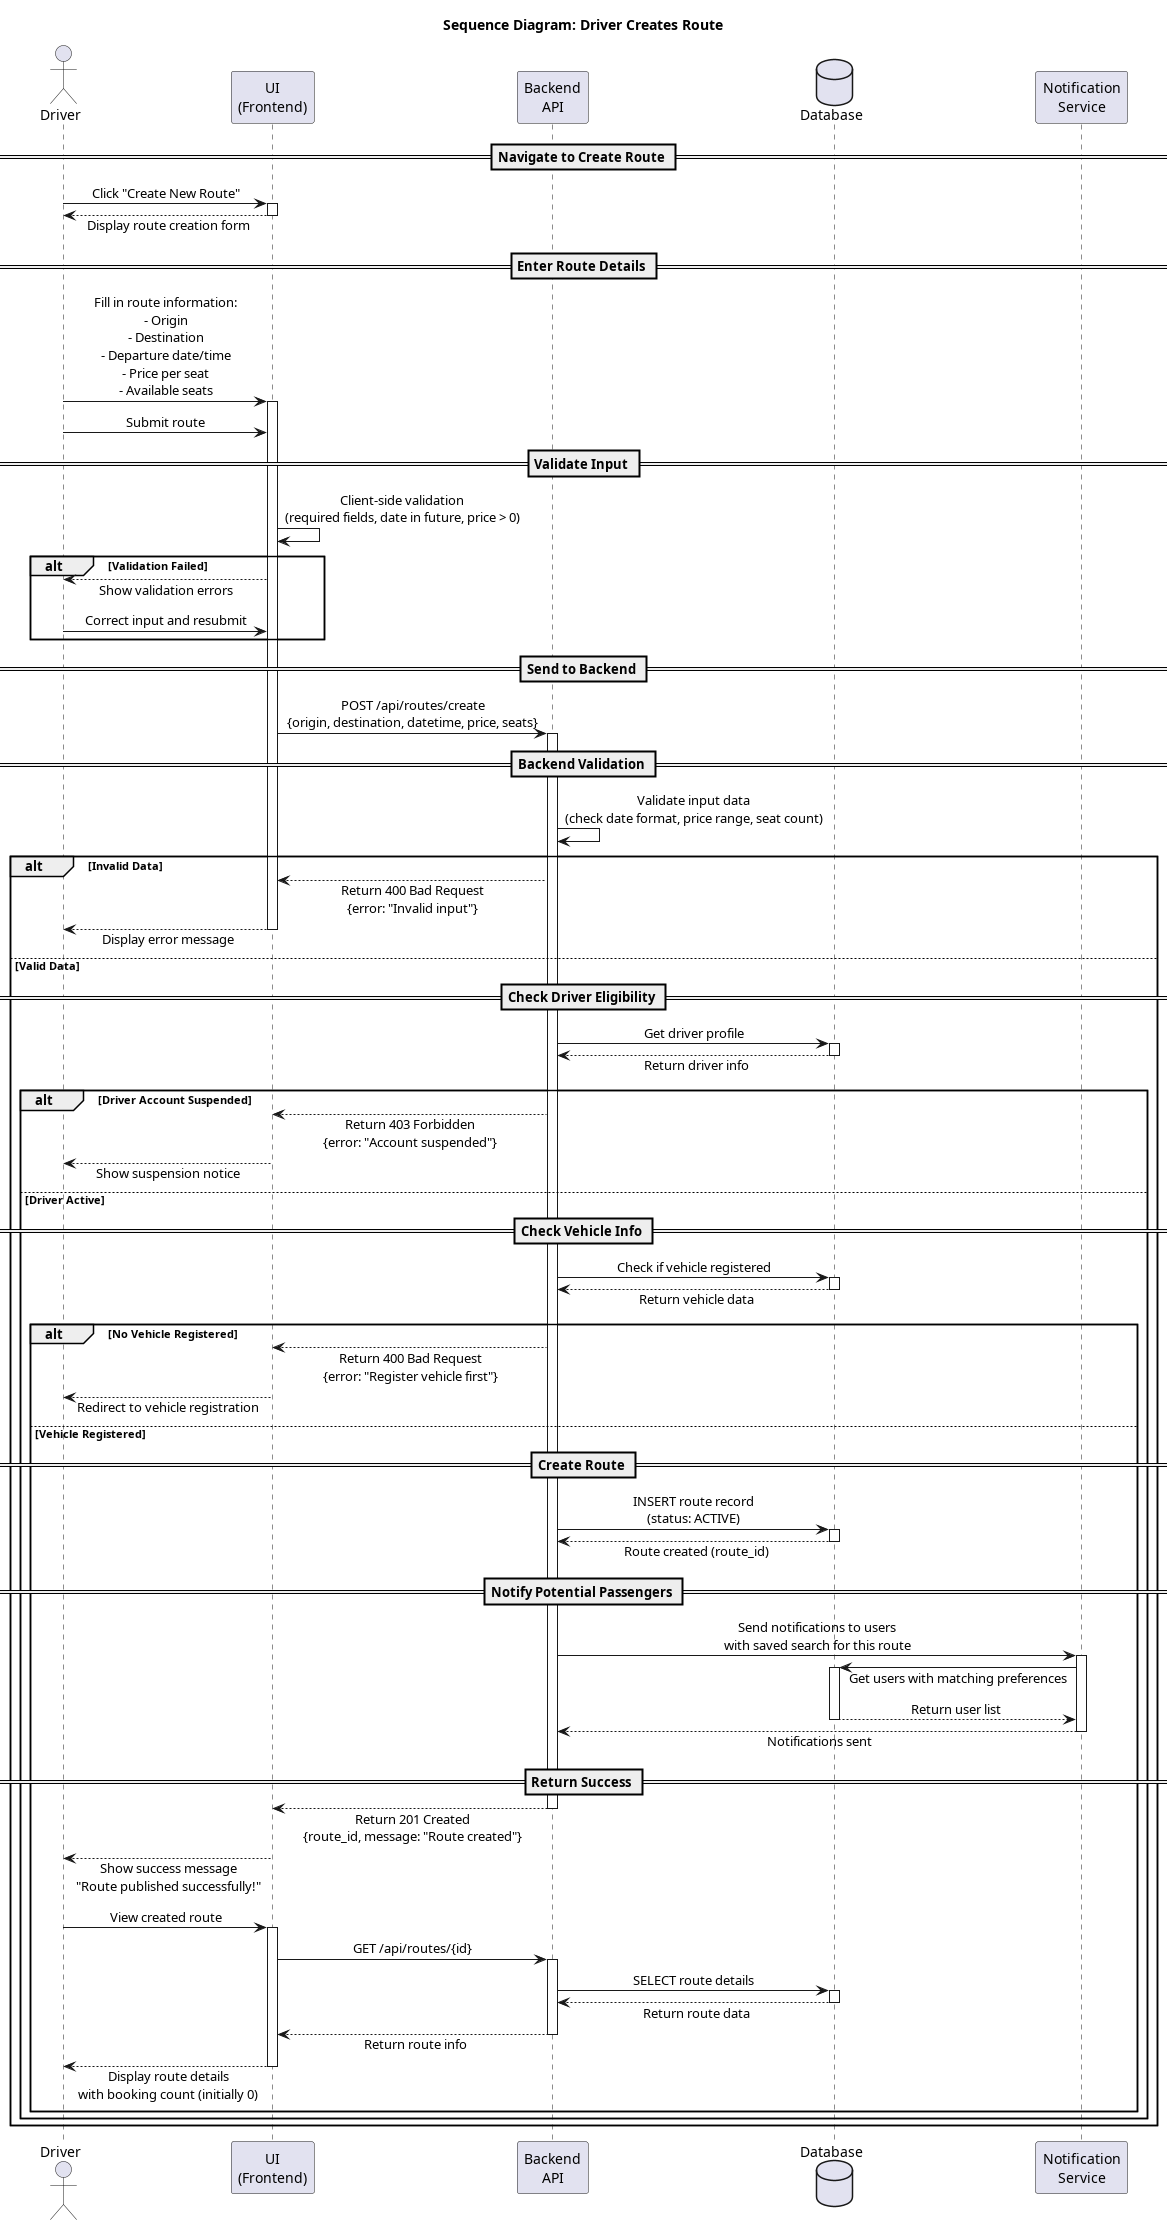
\includegraphics[width=\textwidth, height=0.85\textheight, keepaspectratio]{ForsaDrive_Sequence_CreateRoute.png}
    \caption{Sequence diagram --- driver publishes a route (US2.1)}
    \label{fig:seq_create_route}
\end{figure}

The publication starts with a client-side validation that catches the most common mistakes early. The backend then verifies that the driver account is active, that a vehicle has been registered, and that the requested seat count is consistent with the vehicle. The route is persisted with the status \textit{ACTIVE} and the saved searches that match the new offer trigger a notification.

\begin{figure}[H]
    \centering
    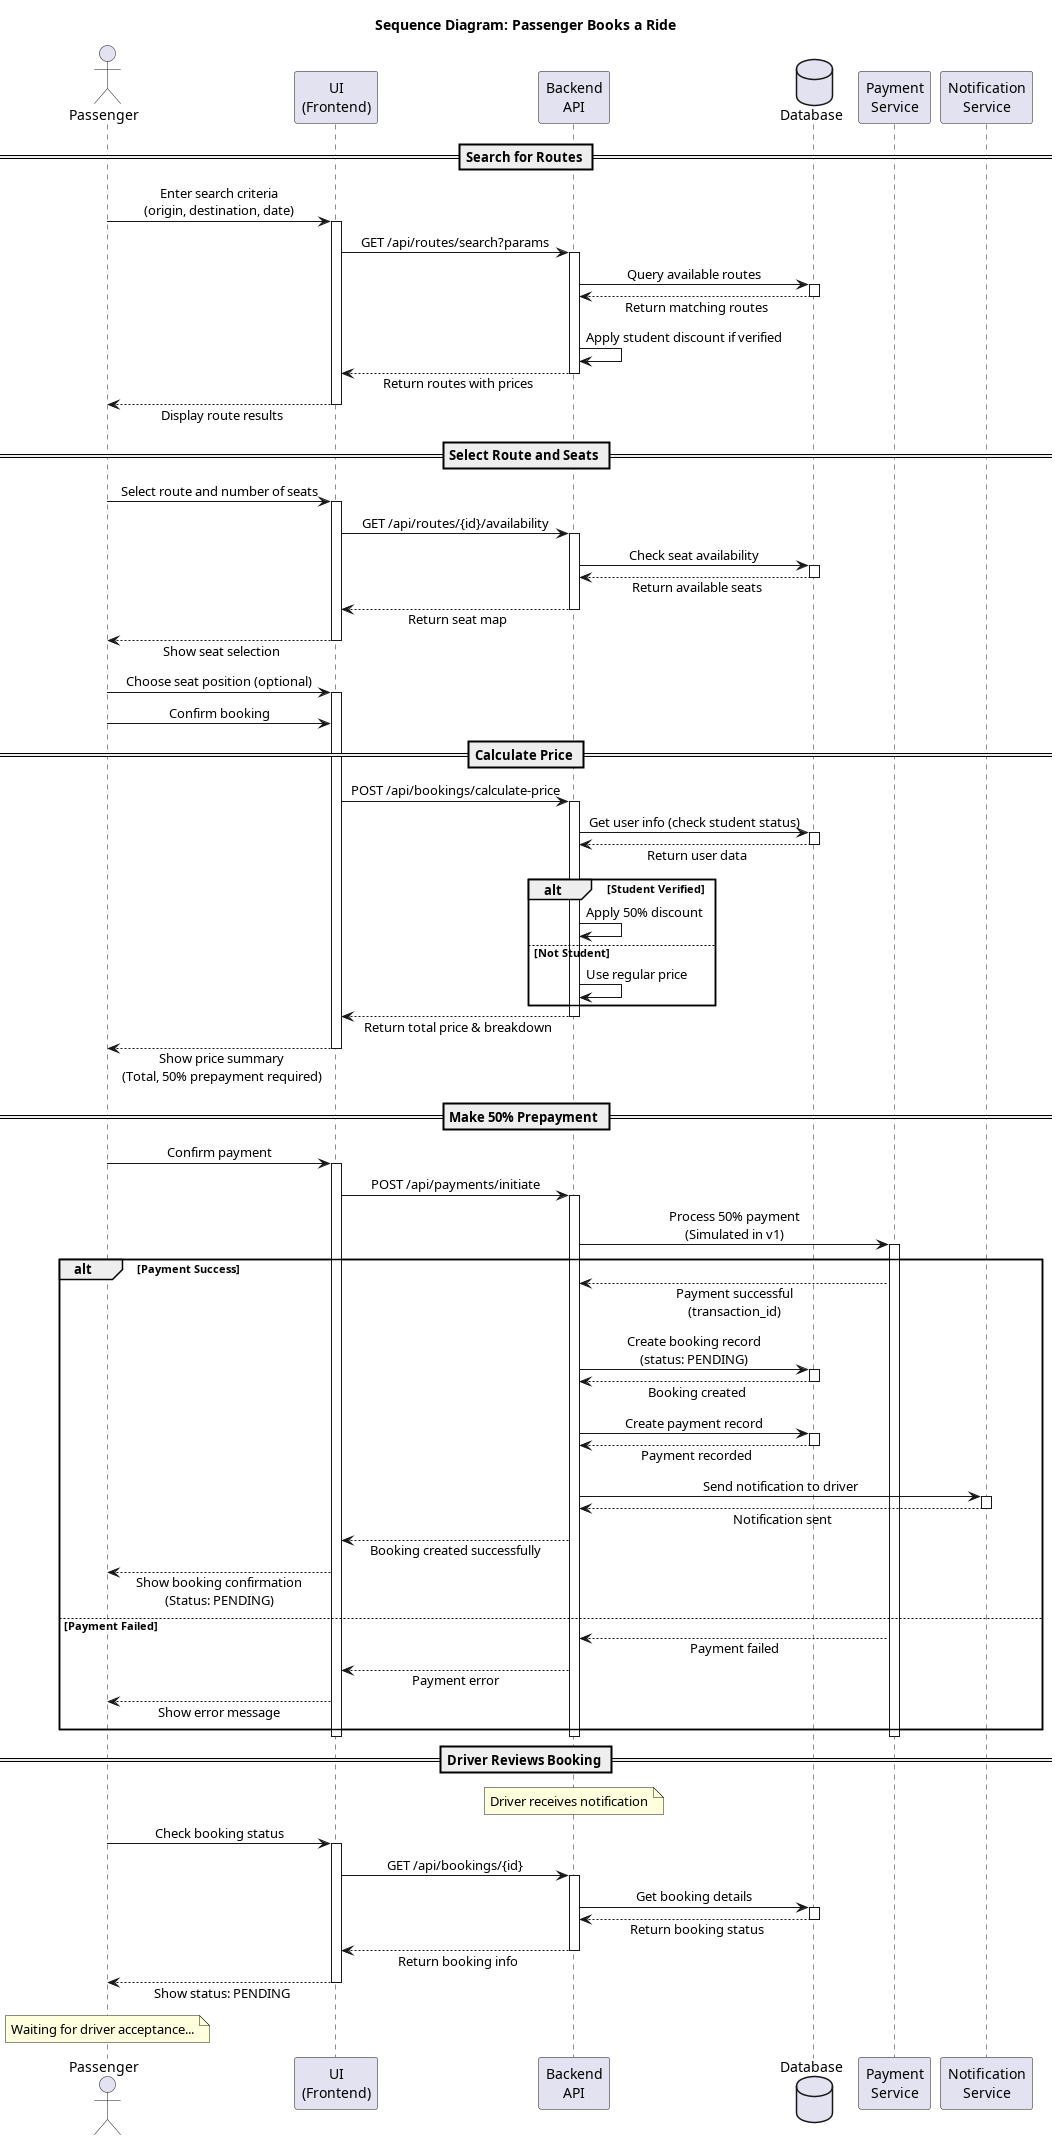
\includegraphics[width=\textwidth, height=0.85\textheight, keepaspectratio]{ForsaDrive_Sequence_BookRide.png}
    \caption{Sequence diagram --- passenger books a ride with prepayment (US2.6)}
    \label{fig:seq_book_ride}
\end{figure}

The booking sequence highlights the interaction between the passenger, the application, the wallet, the notification service, and the database. The student discount is applied at the price computation step, before the prepayment of fifty percent is deducted from the wallet. The booking is only persisted if the deduction succeeds, which guarantees the commitment of the passenger and protects the driver from no-shows.

\begin{figure}[H]
    \centering
    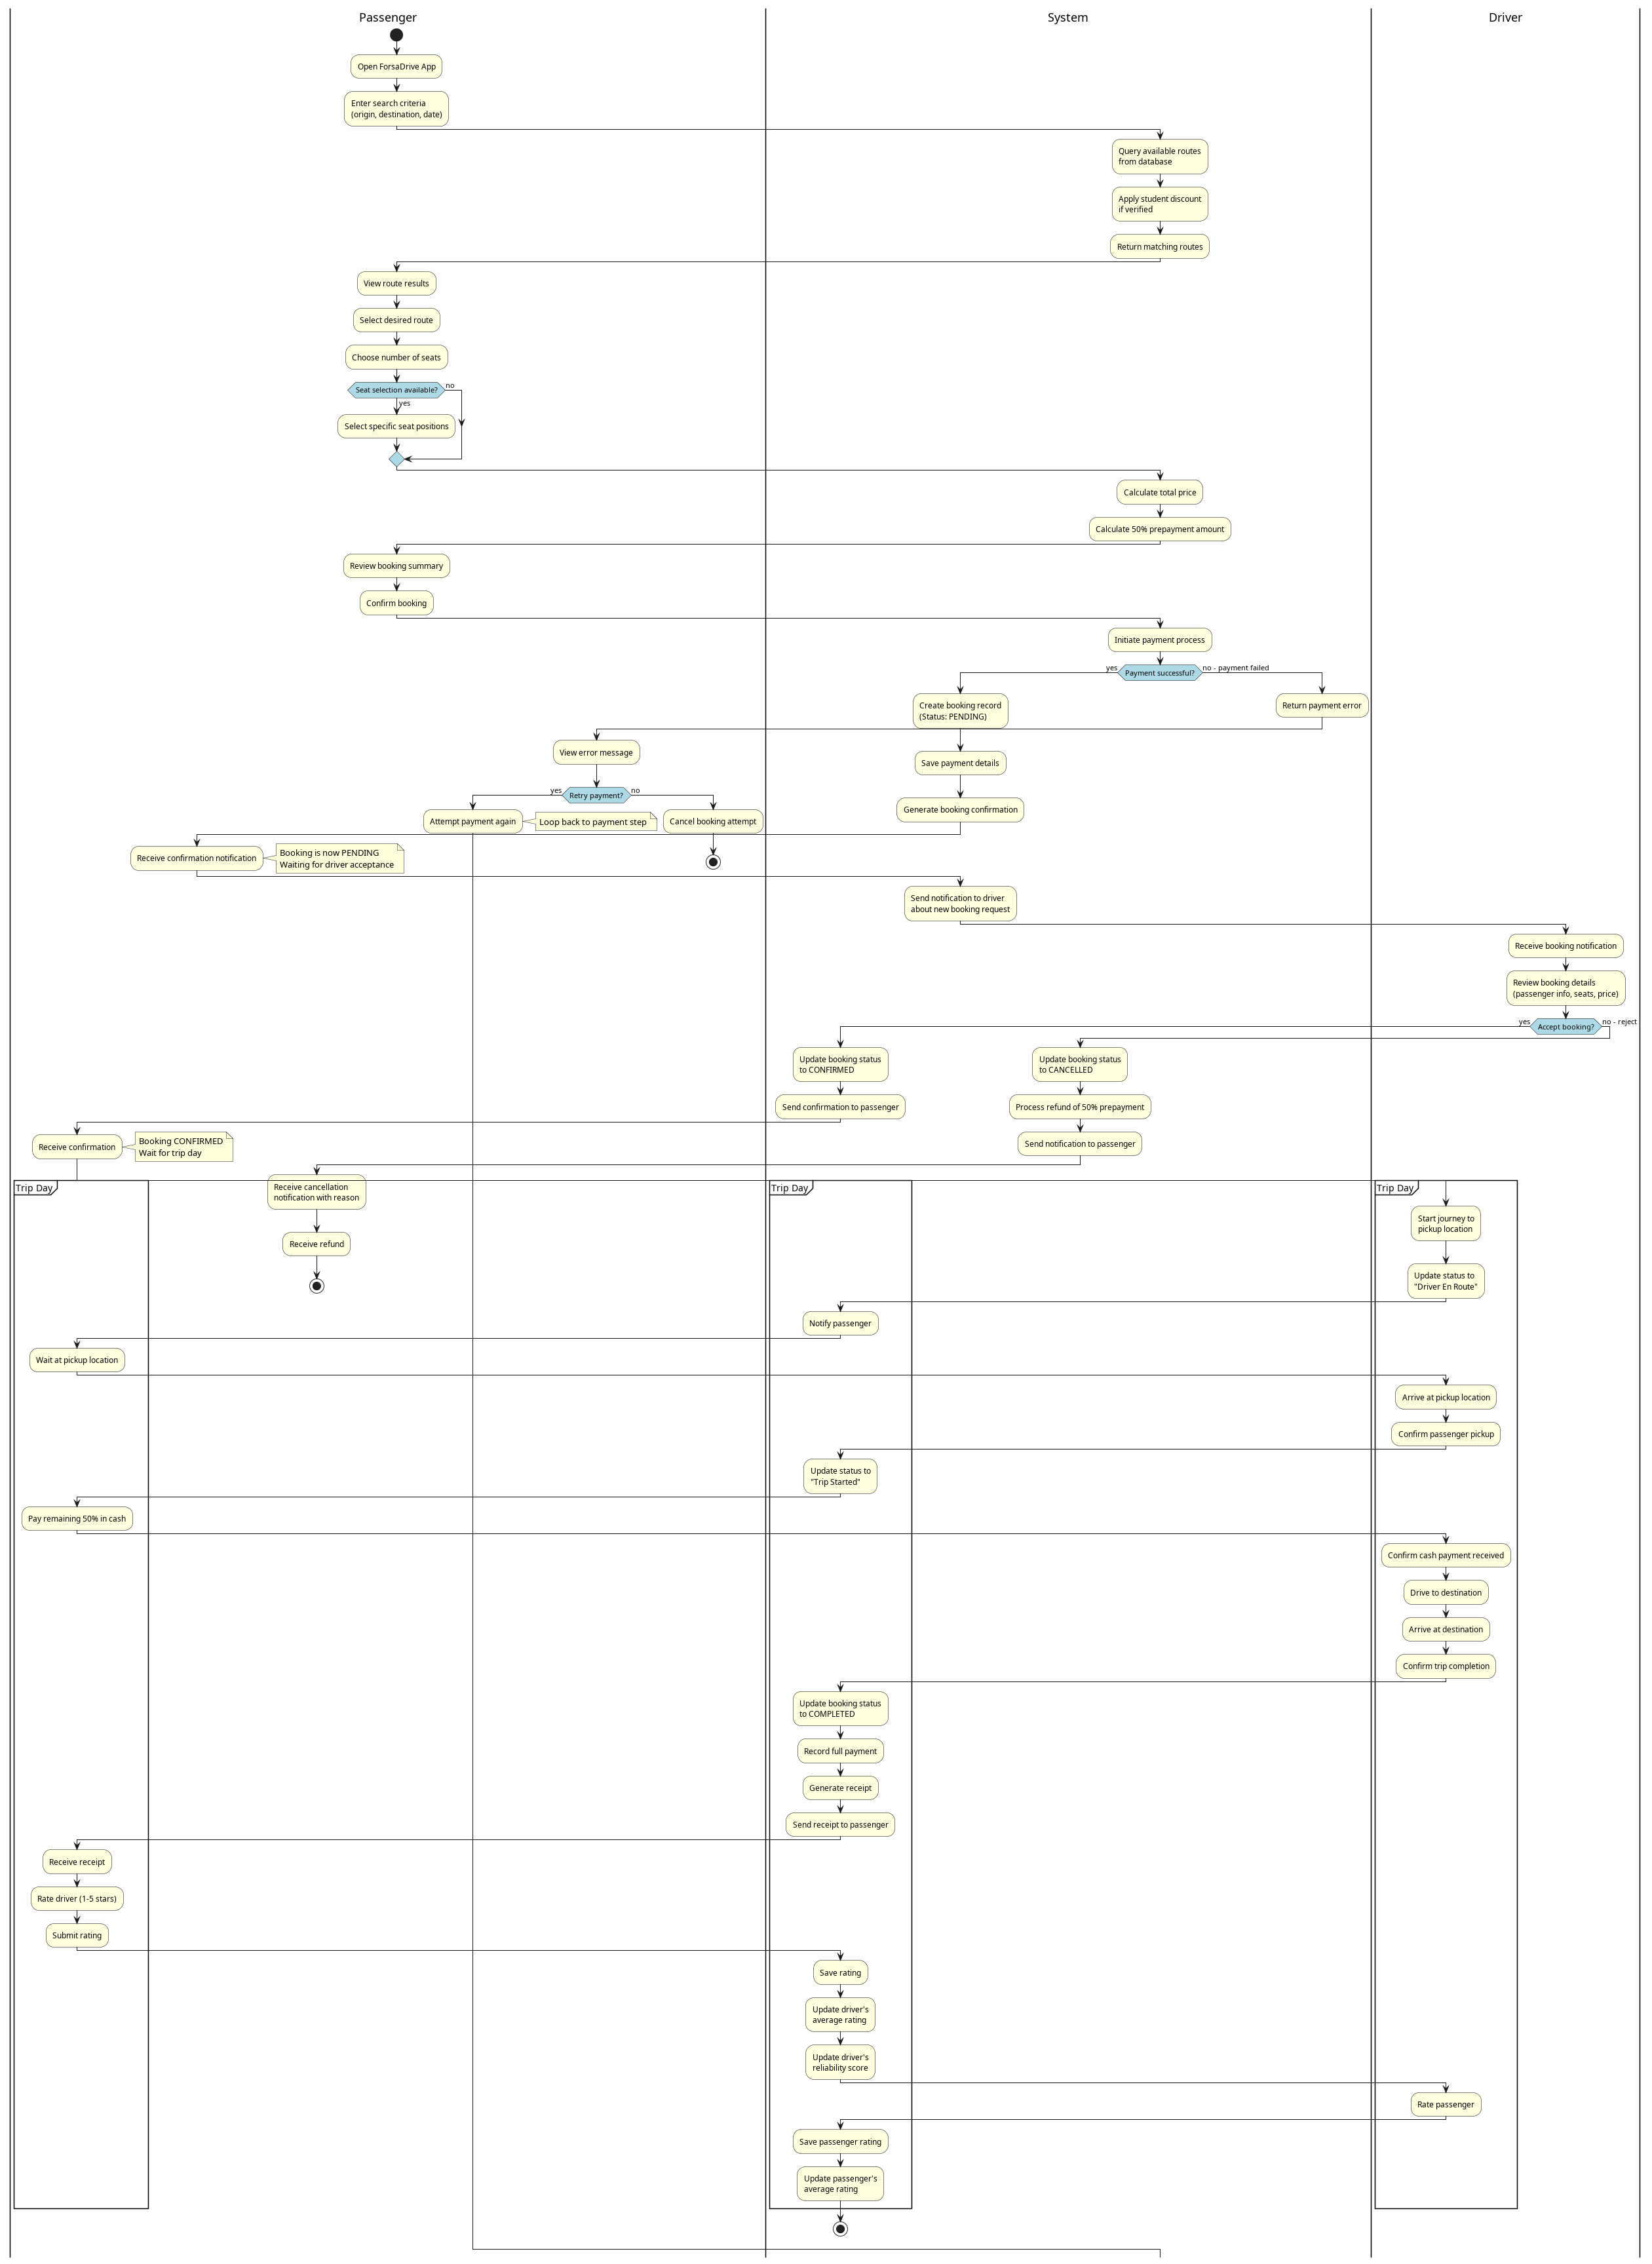
\includegraphics[width=\textwidth, height=0.85\textheight, keepaspectratio]{ForsaDrive_Activity_BookingFlow.png}
    \caption{Activity diagram --- end-to-end booking journey}
    \label{fig:activity_booking_flow}
\end{figure}

The activity diagram complements the sequence diagrams by emphasizing the decision points: the retry of a failed payment, the acceptance or refusal of the booking by the driver, the departure and arrival confirmations, and the cash collection at the end of the trip.

\subsection{Realization}

On the web side, drivers reach the publication form through a dedicated entry in the menu (Figure~\ref{fig:web_publish_trip}). The form requests the mandatory information and shows a preview of how the trip will be displayed to passengers. The search page lets passengers filter trips by origin, destination, date, and preferences, with the results displayed as cards that include the driver's name, the rating, the price, and the remaining seats (Figure~\ref{fig:web_search}). The booking page shows the total amount, the student discount when applicable, and the prepayment, and only confirms the reservation once the prepayment has been registered (Figure~\ref{fig:web_booking}).

\begin{figure}[H]
    \centering
    \includegraphics[width=\textwidth]{web_publish_trip.png}
    \caption{Web --- ride publishing form}
    \label{fig:web_publish_trip}
\end{figure}

\begin{figure}[H]
    \centering
    \includegraphics[width=\textwidth]{web_search.png}
    \caption{Web --- ride search and results}
    \label{fig:web_search}
\end{figure}

\begin{figure}[H]
    \centering
    \includegraphics[width=\textwidth]{web_booking.png}
    \caption{Web --- booking confirmation with prepayment}
    \label{fig:web_booking}
\end{figure}

The mobile application offers the same workflow with a slightly different presentation tailored to the smaller screen. The home screen is centered on a search bar, with a few personalized sections below it that are populated as soon as the user accumulates booking history (Figure~\ref{fig:mobile_home}). The search results screen exposes the same filters as the web side and adds a compatibility score badge on each card, computed from the user's previous bookings and preferences (Figure~\ref{fig:mobile_search}). After selecting a ride, the passenger reaches a detailed view that shows the route on an interactive OpenStreetMap tile, the driver's profile, and the price breakdown including the student discount when applicable. The booking is confirmed after the fifty-percent prepayment is deducted from the wallet (Figure~\ref{fig:mobile_trip_details}).

\begin{figure}[H]
    \centering
    \includegraphics[width=0.55\textwidth]{mobile_home.png}
    \caption{Mobile --- home screen with personalized sections}
    \label{fig:mobile_home}
\end{figure}

\begin{figure}[H]
    \centering
    \includegraphics[width=0.55\textwidth]{mobile_search.png}
    \caption{Mobile --- ride search with filters and match score}
    \label{fig:mobile_search}
\end{figure}

\begin{figure}[H]
    \centering
    \includegraphics[width=0.85\textwidth]{mobile_trip_details.png}
    \caption{Mobile --- trip details with map and booking confirmation}
    \label{fig:mobile_trip_details}
\end{figure}

\subsection{Sprint Review}

The review at the end of Sprint~2 confirmed that the central booking loop was working end to end on both clients. Two adjustments came out of the review and were prioritized for the following sprint: the price filter on the search results was using a fixed maximum of 200~TND, which proved too low for a few long trips, and the group booking flow lacked an explicit confirmation that the passengers traveling together had been informed. The first point was solved by replacing the hard-coded ceiling with a slider whose maximum is computed from the highest ride price in the current result set. The second was deferred to Sprint~4 and ultimately addressed by the in-app chat. The retrospective noted that the time spent on the activity diagram before starting the implementation paid off: the cash collection step, in particular, would otherwise have been forgotten until much later.

\section*{Conclusion}

This chapter reported on the first release of ForsaDrive. Sprint~1 delivered the foundations that every subsequent feature relies on: account creation, authentication, profile management, the self-service student OTP verification, the driver application, and the administrative review that controls access to the driver role. Sprint~2 then built the core interaction loop of the platform, from the publication of a ride to its booking with a fifty-percent prepayment. Together, the two sprints produced an application that already covers the basic carpooling experience and that the team could submit to the supervising engineer for a real demonstration. The next chapter reports on the second release, which adds the wallet, the intelligent features, the community dimension, and the testing and deployment work that closes the project.
